% UTF-8 LaTeX fragment: questions only

\sectionbanner{一、单选题}{共10题，每题5分，共50分}

\begin{question}{1}{5}
6年前，父亲的年龄是儿子的5倍；6年后，父亲的年龄是儿子的3倍。儿子今年多少岁？
\begin{choices}
  \choice{15}
  \choice{18}
  \choice{21}
  \choice{24}
\end{choices}
\end{question}

\begin{question}{2}{5}
有标着\(1,2,3,4,5,6\)的6张数字卡片。每次取两张不同的卡片，分别作为十位和个位，组成一个两位偶数。一共可以组成多少个不同的两位偶数？
\begin{choices}
  \choice{8}
  \choice{12}
  \choice{15}
  \choice{18}
\end{choices}
\end{question}

\begin{question}{3}{5}
在下图中，55个单位正方体被堆叠在一起。将这堆正方体的表面涂色，但与地面接触的底面不涂色。请问将这堆正方体拆开后，共有多少个完全未被涂色的单位正方体？

% Source figure: page-03.png
\begin{center}
\begin{tikzpicture}[
  x={(0.36cm,-0.208cm)},
  y={(-0.36cm,-0.208cm)},
  z={(0cm,0.416cm)},
  line join=miter,
  line cap=butt
]
  \newcommand{\unitcube}[3]{%
    % Right face
    \filldraw[fill=black!18, draw=black, line width=0.85pt]
      (#1+1,#2,#3) -- (#1+1,#2+1,#3) --
      (#1+1,#2+1,#3+1) -- (#1+1,#2,#3+1) -- cycle;
    % Left face
    \filldraw[fill=black!32, draw=black, line width=0.85pt]
      (#1,#2+1,#3) -- (#1+1,#2+1,#3) --
      (#1+1,#2+1,#3+1) -- (#1,#2+1,#3+1) -- cycle;
    % Top face
    \filldraw[fill=black!7, draw=black, line width=0.85pt]
      (#1,#2,#3+1) -- (#1+1,#2,#3+1) --
      (#1+1,#2+1,#3+1) -- (#1,#2+1,#3+1) -- cycle;
  }
  % Back-to-front, bottom-to-top so outlines stay crisp.
  \foreach \k/\off/\n in {0/0/4, 1/0.5/3, 2/1/2, 3/1.5/1, 4/2/0} {
    \foreach \j in {0,...,\n} {
      \foreach \i in {0,...,\n} {
        \unitcube{\i+\off}{\j+\off}{\k}
      }
    }
  }
\end{tikzpicture}
\end{center}

\begin{choices}
  \choice{6}
  \choice{9}
  \choice{13}
  \choice{14}
  \choice{18}
\end{choices}
\end{question}

\begin{question}{4}{5}
小明从甲地到乙地，前一半路程的速度是每小时12千米，后一半路程的速度是每小时18千米。全程的平均速度是多少？
\begin{choices}
  \choice{每小时13.5千米}
  \choice{每小时14.4千米}
  \choice{每小时14千米}
  \choice{每小时15千米}
\end{choices}
\end{question}

\begin{question}{5}{5}
把下面7个图形作为一组，按原顺序不断重复排列：\(\bigcirc,\ \triangle,\ \triangle,\ \square,\ \star,\ \star,\ \square\)。从第1个图形开始计数，第2026个图形是哪个？
\begin{choices}
  \choice{\(\bigcirc\)}
  \choice{\(\star\)}
  \choice{\(\square\)}
  \choice{\(\triangle\)}
\end{choices}
\end{question}

\begin{question}{6}{5}
将4个边长均为\(5\text{ cm}\)且互不重叠的相同正方形，拼成了如下图所示的新图形。求这个新图形的周长。

% Source figure: page-06.png
\begin{center}
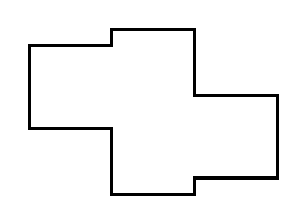
\begin{tikzpicture}[x=1.05cm,y=1.05cm,line width=1.1pt,line join=miter]
  \draw
    (0,0.8) -- (1,0.8) -- (1,1) -- (2,1) -- (2,0.2) --
    (3,0.2) -- (3,-0.8) -- (2,-0.8) -- (2,-1) --
    (1,-1) -- (1,-0.2) -- (0,-0.2) -- cycle;
\end{tikzpicture}
\end{center}

\begin{choices}
  \choice{15}
  \choice{20}
  \choice{30}
  \choice{45}
  \choice{50}
\end{choices}
\end{question}

\begin{question}{7}{5}
在\(1,2,3,\ldots,200\)中，正因数个数为偶数的数有多少个？
\begin{choices}
  \choice{14}
  \choice{180}
  \choice{186}
  \choice{196}
\end{choices}
\end{question}

\begin{question}{8}{5}
从\(1,2,3,\ldots,9\)中等可能地任取两个不同的数，这两个数的乘积是6的倍数的概率是多少？
\begin{choices}
  \choice{\(\dfrac{7}{36}\)}
  \choice{\(\dfrac{1}{3}\)}
  \choice{\(\dfrac{7}{18}\)}
  \choice{\(\dfrac{4}{9}\)}
\end{choices}
\end{question}

\enlargethispage{10mm}
\begin{question}{9}{5}
图中显示了一个带有三个障碍物的\(6\times6\)棋盘。一只蚂蚁在左上角，想要到达右下角。它只能在共用一条边的方格之间爬行，并且只能向下或向右爬行。它不能穿过任何障碍物。请问它共有多少条不同的路径可以走？

% Source figure: page-09.png
{\centering
\vspace{-1mm}
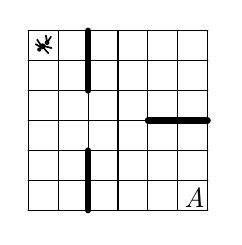
\begin{tikzpicture}[scale=0.38,line cap=round,line join=round]
  \draw[step=1cm,thin] (0,0) grid (6,6);
  % Three impassable barriers.
  \draw[line width=2.2pt] (2,4) -- (2,6);
  \draw[line width=2.2pt] (2,0) -- (2,2);
  \draw[line width=2.2pt] (4,3) -- (6,3);
  % A small vector ant in the upper-left cell.
  \fill (0.48,5.48) circle (0.10);
  \fill (0.63,5.60) circle (0.08);
  \fill (0.37,5.37) circle (0.07);
  \draw[line width=0.6pt]
    (0.43,5.44)--(0.25,5.55)
    (0.44,5.49)--(0.30,5.70)
    (0.52,5.42)--(0.67,5.25)
    (0.56,5.48)--(0.78,5.42)
    (0.67,5.66)--(0.76,5.80)
    (0.62,5.67)--(0.59,5.84);
  \node[font=\itshape] at (5.55,0.42) {A};
\end{tikzpicture}\par}

\begin{choices}
  \choice{88}
  \choice{90}
  \choice{92}
  \choice{96}
  \choice{112}
\end{choices}
\end{question}

\begin{question}{10}{5}
把正整数100写成两个或两个以上正整数之和。在所有写法中，各加数乘积的最大值是多少？
\begin{choices}
  \choice{\(2^{50}\)}
  \choice{\(5^{20}\)}
  \choice{\(2\times3^{33}\)}
  \choice{\(4\times3^{32}\)}
\end{choices}
\end{question}

\sectionbanner{二、填空题}{共5题，每题5分，共25分}

\begin{question}{11}{5}
袋中有3个红球和2个白球，除颜色外完全相同。从中不放回地随机取出2个球。将至少取到1个红球的概率化为最简分数后，分子与分母的和是\answerline
\end{question}

\begin{question}{12}{5}
\[
  1!+2!+3!+\cdots+2026!
\]
除以15的余数是\answerline
\end{question}

\Needspace{6.5cm}
\begin{question}{13}{5}
将四个相同的棋子放入如下图所示黑白相间的\(4\times4\)棋盘中。每个方格最多只能放置一个棋子。所有棋子必须放置在相同颜色的方格中，并且任意两个棋子不能处于同一行或同一列。请问共有多少种不同的放置方法？\answerline

% Source figure: page-13.png
\begin{center}
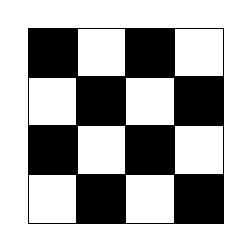
\begin{tikzpicture}[scale=0.62]
  \foreach \r in {0,...,3}{
    \foreach \c in {0,...,3}{
      \pgfmathtruncatemacro{\shadecell}{mod(\r+\c,2)}
      \ifnum\shadecell=0
        \fill[black] (\c,3-\r) rectangle ++(1,1);
      \else
        \fill[white] (\c,3-\r) rectangle ++(1,1);
      \fi
    }
  }
  \draw[step=1cm,thin] (0,0) grid (4,4);
\end{tikzpicture}
\end{center}
\end{question}

\begin{question}{14}{5}
不超过2026且与2026互质的正整数共有\answerline 个。
\end{question}

\begin{question}{15}{5}
参考下图，图中展示了一卷圆柱形的卷筒卫生纸，中间部分由空心纸板卷筒组成。卫生纸被分成若干节，卷在纸板上。包装上标明：“每节\(138\text{ mm}\times100\text{ mm}\)，3层”，这意味着每节长\(138\text{ mm}\)，宽\(100\text{ mm}\)，且包含3层。已知单层卫生纸的厚度为\(0.13\text{ mm}\)，纸板筒的直径为\(5\text{ cm}\)，整卷卫生纸的直径为\(12\text{ cm}\)，请问这一卷中大约有多少节卫生纸（结果四舍五入到整数）？（取\(\pi=3.14\)）

% Source figure: user-provided original — debugged in _q15fig.tex
\noindent
\begin{tikzpicture}[>=Stealth, line cap=round, line join=round, font=\sffamily\small]
  % ===== Left: 3-D horizontal roll =====
  \coordinate (R) at (2.20,3.55);
  \def\rx{0.30}
  \def\ry{0.72}
  \def\len{1.88}
  \coordinate (L) at ($(R)+(-\len,0)$);

  \fill[white]
    ($(L)+(0,-\ry)$) -- ($(R)+(0,-\ry)$)
    -- ($(R)+(0,\ry)$) -- ($(L)+(0,\ry)$) -- cycle;
  \draw[line width=0.9pt] ($(L)+(0,\ry)$) -- ($(R)+(0,\ry)$);
  \draw[line width=0.9pt] ($(L)+(0,-\ry)$) -- ($(R)+(0,-\ry)$);
  \filldraw[fill=white, draw=black, line width=0.9pt]
    (L) ellipse[x radius=\rx, y radius=\ry];
  \filldraw[fill=white, draw=black, line width=0.9pt]
    (R) ellipse[x radius=\rx, y radius=\ry];
  \filldraw[fill=white, draw=black, line width=0.75pt]
    (R) ellipse[x radius=0.10, y radius=0.24];
  \draw[dashed, line width=0.55pt] (L) -- (R);

  \node[align=center] (hc) at ($(R)+(1.55,1.18)$) {Hollow\\Cardboard};
  \draw[line width=0.6pt] ($(R)+(0.95,0.95)$) -- ($(R)+(0.04,0.40)$);

  % Mild trapezoid, dashed "1 sheet" line just under the roll
  \coordinate (STL) at ($(L)+(0.28,-\ry)$);
  \coordinate (STR) at ($(R)+(-0.10,-\ry)$);
  \coordinate (SBL) at ($(STL)+(-0.28,-1.92)$);
  \coordinate (SBR) at ($(STR)+(0.28,-1.92)$);
  \draw[line width=0.85pt] (STL) -- (SBL) -- (SBR) -- (STR);
  \coordinate (SDL) at ($(SBL)!0.88!(STL)$);
  \coordinate (SDR) at ($(SBR)!0.88!(STR)$);
  \draw[dashed, line width=0.55pt] (SDL) -- (SDR);

  \node[draw, rounded corners=4pt, inner xsep=5pt, inner ysep=2.2pt, fill=white] (onesheet)
    at ($(SDL)+(-1.85,0)$) {1 sheet};
  \draw[->, line width=0.7pt] (onesheet.east) -- (SDL);
  \node (threeply) at ($(SBL)+(-1.45,0.04)$) {3 ply};

  % 100 mm: width of the bottom edge
  \draw[<->, line width=0.65pt]
    ([yshift=-3.8mm]SBL) -- ([yshift=-3.8mm]SBR)
    node[midway, below] {\(100\,\mathrm{mm}\)};
  % 138 mm: from the dashed line DOWN to the bottom of the sheet
  \draw[<->, line width=0.65pt]
    ([xshift=4.2mm]SDR) -- ([xshift=4.2mm]SBR)
    node[midway, right] {\(138\,\mathrm{mm}\)};

  % ===== Right: upright roll =====
  \coordinate (U) at (5.85,2.95);
  \def\urx{0.76}
  \def\ury{0.24}
  \def\uh{1.28}
  \def\irx{0.31}

  \draw[line width=0.85pt] ($(U)+(-\urx,0)$) -- ($(U)+(-\urx,-\uh)$);
  \draw[line width=0.85pt] ($(U)+(\urx,0)$) -- ($(U)+(\urx,-\uh)$);
  \draw[line width=0.85pt]
    ($(U)+(-\urx,-\uh)$) arc[start angle=180,end angle=360,x radius=\urx,y radius=\ury];
  \filldraw[fill=white, draw=black, line width=0.85pt]
    (U) ellipse[x radius=\urx, y radius=\ury];
  \filldraw[fill=white, draw=black, line width=0.75pt]
    (U) ellipse[x radius=\irx, y radius=0.10];

  \draw[<->, line width=0.65pt]
    ($(U)+(-\urx,1.18)$) -- ($(U)+(\urx,1.18)$)
    node[midway, above] {\(12\,\mathrm{cm}\)};
  \draw[line width=0.5pt] ($(U)+(-\urx,1.08)$) -- ($(U)+(-\urx,1.28)$);
  \draw[line width=0.5pt] ($(U)+(\urx,1.08)$) -- ($(U)+(\urx,1.28)$);
  \draw[<->, line width=0.65pt]
    ($(U)+(-\irx,0.68)$) -- ($(U)+(\irx,0.68)$)
    node[midway, above] {\(5\,\mathrm{cm}\)};
\end{tikzpicture}

\end{question}

\sectionbanner{三、综合题}{共3题，每题15分，共45分}

\begin{question}{16}{15}
在3000多年前的古埃及，有一份著名的数学文献《莱因德数学纸草书》。考古学家发现，古埃及人对分数有一种奇特的“强迫症”——他们极其偏爱分子为1的分数（例如\(\frac12,\frac13,\frac14\)），我们现在称之为“古埃及分数”。在古埃及人的账本里，任何一个真分数，都必须拆分成几个“古埃及分数”相加的形式。为了完成这种拆分，古埃及大祭司们定下了两条极其严格的铁律：

铁律1：拆分出来的所有分数，分子必须全都是1。

铁律2：拆分出来的分数，分母绝对不能重复！（例如：把\(\frac35\)写成\(\frac15+\frac15+\frac15\)是犯法的，因为分母重复了！）

那么，古埃及人是怎么把\(\frac35\)这样分子不是1的分数拆开，又不违反规则的呢？聪明的大祭司发明了一个“魔法拆分公式”：他们发现，任何一个分子为1的分数，都可以裂变成两个更小的、且分母不同的古埃及分数。公式如下：
\[
  \frac1n=\frac1{n+1}+\frac1{n\times(n+1)}
\]
（注：\(n\)代表同一个非零自然数）

【魔法演示】假设我们要拆分\(\frac13\)（此时公式里的\(n=3\)）：
\[
  \frac13=\frac1{3+1}+\frac1{3\times(3+1)}
  =\frac14+\frac1{12}.
\]
你看！\(\frac13\)成功变成两个不同的古埃及分数相加，并且验证一下：
\[
  \frac14+\frac1{12}=\frac3{12}+\frac1{12}
  =\frac4{12}=\frac13,
\]
完全正确！

\subquestion{5}{古埃及法老要求把\(\frac34\)块黄金分给大臣。以下四位学者的拆分方案中，哪一个完全符合古埃及分数的“两条铁律”？}
\begin{choices}
  \choice{\(\dfrac34=\dfrac14+\dfrac14+\dfrac14\)}
  \choice{\(\dfrac34=\dfrac12+\dfrac14\)}
  \choice{\(\dfrac34=\dfrac24+\dfrac14\)}
  \choice{\(\dfrac34=\dfrac13+\dfrac13+\dfrac1{12}\)}
\end{choices}

\subquestion{5}{请你模仿材料中的“魔法拆分公式”，把\(\frac16\)拆分成两个不同的古埃及分数相加。}
\[
  \frac16=\frac1{(\quad)}+\frac1{(\quad)}
\]
（注意：请在括号内填入适当的纯数字，且要求第一个括号里的数字比第二个括号里的数字小）请问第二个括号里应该填写的数字是？
\answerspace

\subquestion{5}{前面提到，古埃及人不能把\(\frac25\)直接写成\(\frac15+\frac15\)。现在，请你利用刚才学到的所有知识，帮古埃及人把\(\frac25\)拆分成三个完全不同的古埃及分数相加。}
\[
  \frac25=\frac1{(\quad)}+\frac1{(\quad)}+\frac1{(\quad)}
\]
（提示：你可以先暂时把它写成\(\frac15+\frac15\)，然后对其中一个\(\frac15\)使用魔法拆分公式！请按照数字从小到大的顺序填写分母）请问最后一个空应该填写几？
\answerspace
\end{question}

\begin{question}{17}{15}
如图1所示，考虑在边长为\(1\text{ cm}\)的正六边形\(ABCDEF\)内部沿直线运动的点\(P\)的轨迹。当点\(P\)到达边界（边）时，会如图2所示发生反弹（注：入射角等于反射角）。但是，若点\(P\)恰好到达正六边形的顶点，则会在该顶点处停止运动。现已知点\(P\)从顶点\(A\)出发，且其轨迹的第一次反弹发生在边\(CD\)上的某一点。请回答下列问题。请根据上述规则回答以下问题：

% Source figures: page-19.png
\begin{center}
\begin{tikzpicture}[>=Stealth,line cap=round,line join=round]
  \begin{scope}[xshift=-3.2cm,scale=1.55]
    \coordinate (A) at (0,1);
    \coordinate (B) at (-0.866,0.5);
    \coordinate (C) at (-0.866,-0.5);
    \coordinate (D) at (0,-1);
    \coordinate (E) at (0.866,-0.5);
    \coordinate (F) at (0.866,0.5);
    \coordinate (X) at (-0.30,-0.827);
    \coordinate (P) at (0.03,-0.52);
    \draw (A)--(B)--(C)--(D)--(E)--(F)--cycle;
    \draw (A)--(X);
    \draw[->] (X)--(P);
    \node[above] at (A) {\(A\)};
    \node[left] at (B) {\(B\)};
    \node[left] at (C) {\(C\)};
    \node[below] at (D) {\(D\)};
    \node[right] at (E) {\(E\)};
    \node[right] at (F) {\(F\)};
    \node[above right] at (P) {\(P\)};
    \node at (0,-1.45) {图1};
  \end{scope}

  \begin{scope}[xshift=2.3cm,yshift=-0.35cm]
    \node[align=center] at (0,2.25) {使做了标记的两个角大小相等地反弹。};
    \draw (-1.65,0)--(1.65,0);
    \draw (-1.50,1.80)--(0,0);
    \draw[->] (0,0)--(0.78,1.02);
    \draw (0,0) ++(180:0.43)
      arc[start angle=180,end angle=130,radius=0.43];
    \draw (0,0) ++(0:0.43)
      arc[start angle=0,end angle=53,radius=0.43];
    \node at (0,-0.48) {图2};
  \end{scope}
\end{tikzpicture}
\end{center}

\subquestion{5}{在边\(CD\)上完成第一次反弹后，点\(P\)接下来可能到达的边有哪些？}
\begin{choices}
  \choice{边\(AB\)和边\(BC\)}
  \choice{边\(BC\)和边\(DE\)}
  \choice{边\(AF\)和边\(EF\)}
  \choice{边\(AB\)和边\(AF\)}
\end{choices}

\subquestion{5}{若点\(P\)首先在边\(CD\)上的点\(X\)处发生反弹，在接下来到达的边上又发生了1次反弹（共反弹2次），最终恰好到达了顶点\(D\)。求线段\(CX\)的长度。}
\begin{choices}
  \choice{\(\dfrac14\text{ cm}\)}
  \choice{\(\dfrac13\text{ cm}\)}
  \choice{\(\dfrac12\text{ cm}\)}
  \choice{\(\dfrac23\text{ cm}\)}
\end{choices}

\subquestion{5}{若点\(P\)首先在边\(CD\)上的点\(Y\)处发生反弹，接着又连续发生了2次反弹（共反弹3次），最终恰好到达了顶点\(D\)。求线段\(CY\)的长度。}
\begin{choices}
  \choice{\(\dfrac35\text{ cm}\)}
  \choice{\(\dfrac47\text{ cm}\)}
  \choice{\(\dfrac57\text{ cm}\)}
  \choice{\(\dfrac58\text{ cm}\)}
\end{choices}
\end{question}

\begin{question}{18}{15}
袋子里装有写着数字1、2、3的卡片各若干张。每次从袋子中随机抽取1张卡片，确认上面的数字后，再将卡片放回袋中。按照抽出卡片上的数字，在方格地图上前进相应的步数。从“起点”出发，重复此抽卡前进的操作，请回答以下问题：

\subquestion{5}{若终点设定为第4格，恰好停在第4格的走法共有多少种？（\quad）}
\begin{choices}
  \choice{4}
  \choice{6}
  \choice{7}
  \choice{8}
\end{choices}

\subquestion{5}{若终点设定为图中的第10格，恰好停在第10格的走法共有多少种？（仅填写数字）}
\answerspace

\subquestion{5}{在第2问（走到第10格）的所有走法中，要求中途必须恰好停在第6格，符合条件的走法共有多少种？（仅填写数字）}
\answerspace
\end{question}
